%\documentclass[show notes]{beamer}       % print frame + notes
\documentclass[11pt,handout]{beamer}   % only notes
%\documentclass[aspectratio=169]{beamer}              % only frames

\definecolor{DarkGray}{HTML}{63656a}
\setbeamertemplate{note page}[plain]
\setbeamertemplate{navigation symbols}{}
\setbeamertemplate{footline}[text line]{%
    \hfill\strut{\scriptsize\sf\color{DarkGray}\today}\hfill\strut{%
        \scriptsize\sf\color{DarkGray}%
        \quad\insertframenumber/\inserttotalframenumber
    }%
}

\beamertemplatenavigationsymbolsempty

\title[Your Short Title]{Nonlinear Control Systems}
\subtitle{Lsn 1: Introduction}
\author{I. Weintraub, Dr. Cobb, \& Capt. Hess}
\institute{Air Force Institute of Technology}
\date{\today}

\begin{document}

\begin{frame}
  \titlepage
\end{frame}

\begin{frame}
\frametitle{Syllabus}
    Description
    \begin{itemize}
      \item This course serves as an introduction to the fundamental results of modern and nonlinear control. 
      \item The first half of this course will concentrate on the analytical tools that can be used to study a nonlinear system. Specific topics in this area are phase-plane analysis, stability, Lyapunov theory, perturbation methods, and describing function.
    \item The second half of this course will cover several nonlinear control sythesis techniques such as feedback linearization, sliding mode, and model reference adaptive control.
    \end{itemize}
\end{frame}

\begin{frame}
\frametitle{Syllabus}
	\textbf{Instructors}\\
    Dr. Richard Cobb and Capt. Joshua Hess\\
	\textbf{References}\\
 	\begin{itemize}
 	\item Applied Nonlinear Control, Slotine ad Li
    \item Nonlinear Systems, Khalil
    \item Nonlinear Systems, Sastry
    \item ASYS 625 Course Notes
    \item Additional reference materials as needed
 	\end{itemize}
\end{frame}

\begin{frame}
\frametitle{Calendar}
\begin{table}
\centering
    \begin{tabular}{l  c}
    \hline
    Timeline & Topic \\ \hline
    Week 1 & Introduction and Math Review\\
    Week 1-2 & Phase Plane Analysis\\
    Week 2-4 & Fundamentals of Lyapunov Theory\\
    Week 4   & Advanced Stability Theory\\
    Week 4-5 & Describing Functions \\
    Week 5-7 & Feedback Linearizion \\ 
    Week 8-9 & Sliding Mode Control \\
    Week 10  & Adaptive Control \\\hline
    \end{tabular}
\end{table}
\end{frame}
 
\begin{frame}
\frametitle{Nonlinear Control}
\textbf{Nonlinear Control} deals with the analysis and design of nonlinear control systems. Slotine and Li state this process of designing a nonlinear control system is completed in two parts:
\begin{enumerate}
\item Analysis
\item Design
\end{enumerate}

\begin{columns}[T] % align columns
\begin{column}{.48\textwidth}
\textbf{Analysis}\\ 
A nonlinear closed-loop system is assumed to have been designed and we wish to determine the characteristics of the system's behavior 
\end{column}%
\hfill%
\begin{column}{.48\textwidth}
\textbf{Design}\\ 
Given a nonlinear plant to be controlled and some specifications of closed-loop system behavior, our task is to construct a controller so that the closed-loop system meets the desired characteristics.
\end{column}%
\end{columns}
\end{frame}

\begin{frame}
\frametitle{Reasons Cited for Nonlinear Control}
\begin{itemize}
\item Improvement of existing control systems
\begin{itemize}
\item linear control methods rely on assumptions
\item nonlinear controllers can out perform linear controllers for nonlinear plants when ``large range'' operation is required
\end{itemize}
\item Analysis of hard non-linearities
\begin{itemize}
\item Hard nonlinearities including coulomb friction, saturation, dead-zones, backlash, and hysteresis are common in engineering and can not be linearized
\item Undesirable behaviors result from ``hard nonlinearities''
\end{itemize}
\item Dealing with model uncertainties
\begin{itemize}
\item Many control problems involve uncertainties in the model
\item Robust and Adaptive controllers are classes of non-linear controllers that may address model changes or uncertainties.
\end{itemize}
\item Design simplicity
\begin{itemize}
\item Simpler methods/algorithms rather than gain scheduling or linearizing about many points
\item Nonlinear control can be more intuitive than an implementation of linear control to a nonlinear problem
\end{itemize}
\end{itemize}
\end{frame}

\begin{frame}
\frametitle{Nonlinear System Behavior}
\textbf{Types of Nonlinearities}
\begin{enumerate}
\item Inherent 
\item Intentional
\end{enumerate}

\textbf{Inherent} nonlinearities are those which naturally come with the system's hardware and motion.\\
\begin{itemize}
\item Centripetal Forces
\item Coulomb Friction
\end{itemize}
\textbf{Intentional} nonlinearities are those which are introduced by the designer.\\
\begin{itemize}
\item Adaptive Control Laws
\item Bang-Bang Optimal Control Laws
\end{itemize}
\end{frame}


\begin{frame}
\frametitle{Nonlinear System Example}
\textbf{Underwater Vehicle}
\begin{equation}
\dot{v} + |v|v = u(t)
\end{equation}
$v$ is the velocoty of the vehicle\\
$u(t)$ is the input ``thrust''\\
\textbf{Case 1: Input of 1.0}\\
\begin{equation*}
\begin{aligned}
v s + |v|v &=& 1.0\\
|v_{\infty}|v_{\infty} &=& 1.0\\
\therefore v_{\infty} = \sqrt{1} &=& 1.0
\end{aligned}
\end{equation*}
\textbf{Case 2: Input of 10.0}\\
\begin{equation*}
\begin{aligned}
v s + |v|v &=& 10.0\\
|v_{\infty}|v_{\infty} &=& 10.0\\
\therefore v_{\infty} = \sqrt{10.0} &\approx& 3.16
\end{aligned}
\end{equation*}
\end{frame}

\begin{frame}
\frametitle{Nonlinear System Example}
\begin{figure}
\centering
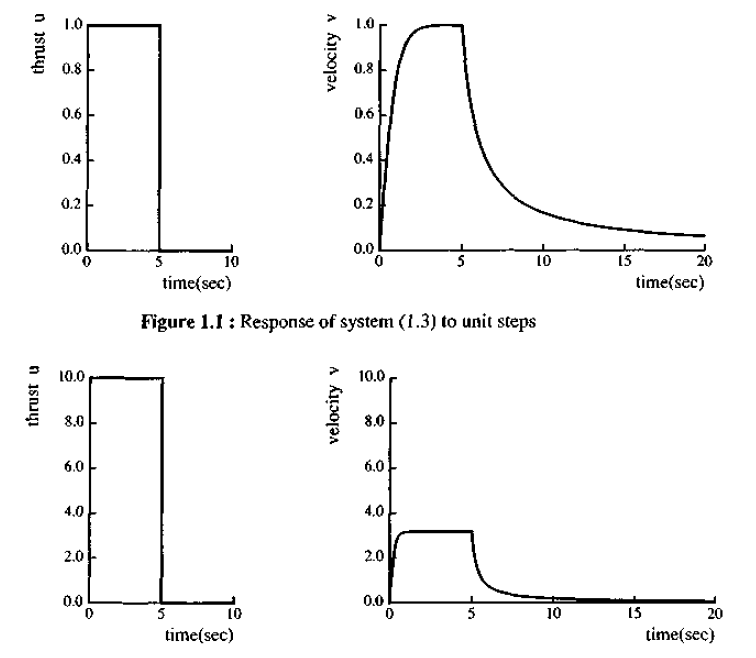
\includegraphics[width = 3in]{NonLinearExample_1.PNG}
\end{figure}
Slotine and Li pg. 6
\end{frame}

\begin{frame}
\frametitle{Common Nonlinear System Behaviors}

\begin{itemize}
\item \textbf{Multiple Equilibrium Points} A point where a system can stay forever without moving
\item \textbf{Limit Cycles} A self excited oscillation. An example displays oscillations of fixed amplitude or frequency without externalization excitation.
\item \textbf{Bifurcations} As parameters of a nonlinear system change so can the stability of equilibrium points as well as the number of equilibrium points.
\item \textbf{Chaos} A system output is extremely sensitive to the initial conditions. The essential feature of chaos is the unpredictability of the system output.
\item Other...
\end{itemize}
\end{frame}


\begin{frame}
\frametitle{Nonlinear Systems Analysis}
\textbf{Why Study of Nonlinear Analysis Techniques?}
\begin{itemize}
\item Theoretical Analysis is very inexpensive
\item Simulations are guided by theory
\item Design of nonlinear controllers are based upon analysis
\item Analysis tools allow us to assess control designs after they have been made
\item Direct solutions of nonlinear differential equations is generally impossible and frequency domain transformations don't apply.
\end{itemize}
\Large{\textit{The standard time and frequency tools used for linear control do not apply to nonlinear systems} - Slotine \& Li}
\end{frame}

\begin{frame}
\frametitle{Nonlinear Systems Analysis}
\textbf{Phase Plane Analysis}\\
\begin{itemize}
\item A graphical method of studying 2nd order nonlinear systems
\item Solve a 2nd order differential equation grpahically instead of seeking an analytical solution
\item It provides intuitive insight about nonlinearities
\end{itemize}
\textbf{Lyapunov Theory}\\
\begin{itemize}
\item \textbf{Indirect Method} states that stability properties of a nonlinear system is the close vicinity of an equilibrium point are essentially the same as those of its linearized approximation.
\item \textbf{Direct Method} A generalization of the energy concepts associated with mechanical systems. \textit{The motion of a mechanical system is \underline{stable} if its total mechanical energy decreases all the time}
\end{itemize}
\end{frame}

\begin{frame}
\frametitle{Nonlinear Systems Analysis}
\textbf{Lyapunov Theory General Process:}
\begin{enumerate}
\item Formulate a scalar positive function of the system states
\item Choose a control law to make this function decrease
\item Stable Nonlinear Control System
\end{enumerate}
\textbf{Describing Functions}
\begin{itemize}
\item An approximate technique for studying nonlinear systems
\item Approximate the nonlinear components in nonlinear control systems by linear ``equivalents,'' and then use frequency domain techniques.
\item Less guess and check compared to Lyapunov Direct Method
\end{itemize}
\end{frame}

\end{document}